Certainly! Below is a TikZ LaTeX code snippet that represents a Deterministic Finite Automaton (DFA) \( T_i \) for computing the sequence-to-sequence language \( g(w', p) = I_{L_{\texttt{swap}(p,i)}}(w') \) where \( i = 3 \). The symbols \(\sigma\) and \(\sigma'\) refer to any symbol in \(\Sigma\) and \(\Sigma_{\#}\), respectively.

```latex
\documentclass{article}
\usepackage{tikz}
\usetikzlibrary{automata, positioning}

\begin{document}

\begin{figure}[h]
    \centering
    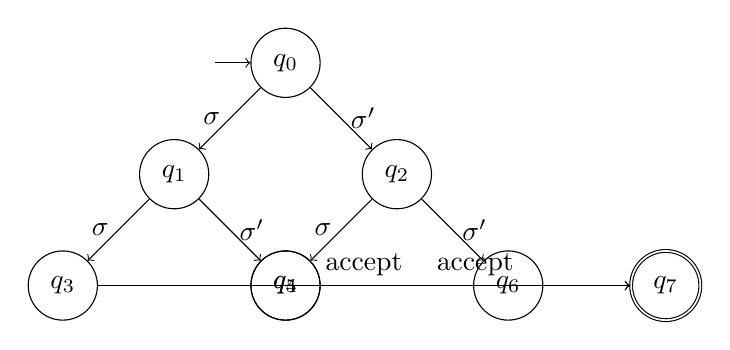
\begin{tikzpicture}[node distance=2cm, auto]
        % Nodes
        \node[state] (q0) [initial, initial text={}] {$q_0$};
        \node[state] (q1) [below left of=q0] {$q_1$};
        \node[state] (q2) [below right of=q0] {$q_2$};
        \node[state] (q3) [below left of=q1] {$q_3$};
        \node[state] (q4) [below right of=q1] {$q_4$};
        \node[state] (q5) [below left of=q2] {$q_5$};
        \node[state] (q6) [below right of=q2] {$q_6$};

        % Edges
        \path[->]
            (q0) edge node[left] {\(\sigma\)} (q1)
                 edge node[right] {\(\sigma'\)} (q2)
            (q1) edge node[left] {\(\sigma\)} (q3)
                 edge node[right] {\(\sigma'\)} (q4)
            (q2) edge node[left] {\(\sigma\)} (q5)
                 edge node[right] {\(\sigma'\)} (q6);

        % Accept states
        \node[state, accepting] (q7) [right of=q6] {$q_7$};

        % Edges to accept state
        \path[->]
            (q3) edge node[above] {accept} (q7)
            (q5) edge node[above] {accept} (q7);
    \end{tikzpicture}
